% Straight up stealing preamble from Eli Holmes 
%%%%%%%%%%%%%%%%%%%%%%%%%%%%%%%%%%%%%%START PREAMBLE THAT IS THE SAME FOR ALL EXAMPLES
\documentclass{article}

%Required: You must have these
\usepackage{Sweave}
\usepackage{graphicx}
\usepackage{tabularx}
\usepackage{hyperref}
\usepackage{natbib}
\usepackage{pdflscape}
\usepackage{array}
\usepackage{gensymb}

%\usepackage[backend=bibtex]{biblatex}
%Strongly recommended
 %put your figures in one place
 
%you'll want these for pretty captioning
\usepackage[small]{caption}

\setkeys{Gin}{width=0.8\textwidth} %make the figs 50 perc textwidth
\setlength{\captionmargin}{30pt}
\setlength{\abovecaptionskip}{0pt}
\setlength{\belowcaptionskip}{10pt}
% manual for caption http://www.dd.chalmers.se/latex/Docs/PDF/caption.pdf

%Optional: I like to muck with my margins and spacing in ways that LaTeX frowns on
%Here's how to do that
 \topmargin -2cm     
 \oddsidemargin -0.04cm   
 \evensidemargin -0.04cm  % same as oddsidemargin but for left-hand pages
 \textwidth 16.59cm
 \textheight 22.94cm 
 %\pagestyle{empty}       % Uncomment if don't want page numbers
 \parskip 7.2pt           % sets spacing between paragraphs
 %\renewcommand{\baselinestretch}{1.5} 	% Uncomment for 1.5 spacing between lines
\parindent 0pt% sets leading space for paragraphs
\usepackage{setspace}
%\doublespacing

%Optional: I like fancy headers
\usepackage{fancyhdr}
\pagestyle{fancy}
\fancyhead[LO]{Ettinger et al. Appendix S1.}
\fancyhead[RO]{2017}

%%%%%%%%%%%%%%%%%%%%%%%%%%%%%%%%%%%%%%END PREAMBLE THAT IS THE SAME FOR ALL EXAMPLES

%Start of the document
\begin{document}

% \SweaveOpts{concordance=TRUE}
\bibliographystyle{/Users/aileneettinger/citations/Bibtex/styles/amnat.bst}
\title{Ettinger et al. American Journal of Botany. 2018. Appendix S1.} 
\author{A.K. Ettinger, S. Gee, and E.M. Wolkovich}
%\date{\today}
\maketitle  %put the fancy title on
%\tableofcontents      %add a table of contents
%\clearpage
%%%%%%%%%%%%%%%%%%%%%%%%%%%%%%%%%%%%%%%%%%%%%%%%%%%
\renewcommand{\thefigure}{S\arabic{figure}}


%\section*{Supplemental Methods}

%\section* {Supplemental Results}


%\section{Bibliography}
%\bibliography{/Users/aileneettinger/citations/Bibtex/mylibrary}



%\section* {Supplemental Figures}

\begin{figure}[h]
  \centering
  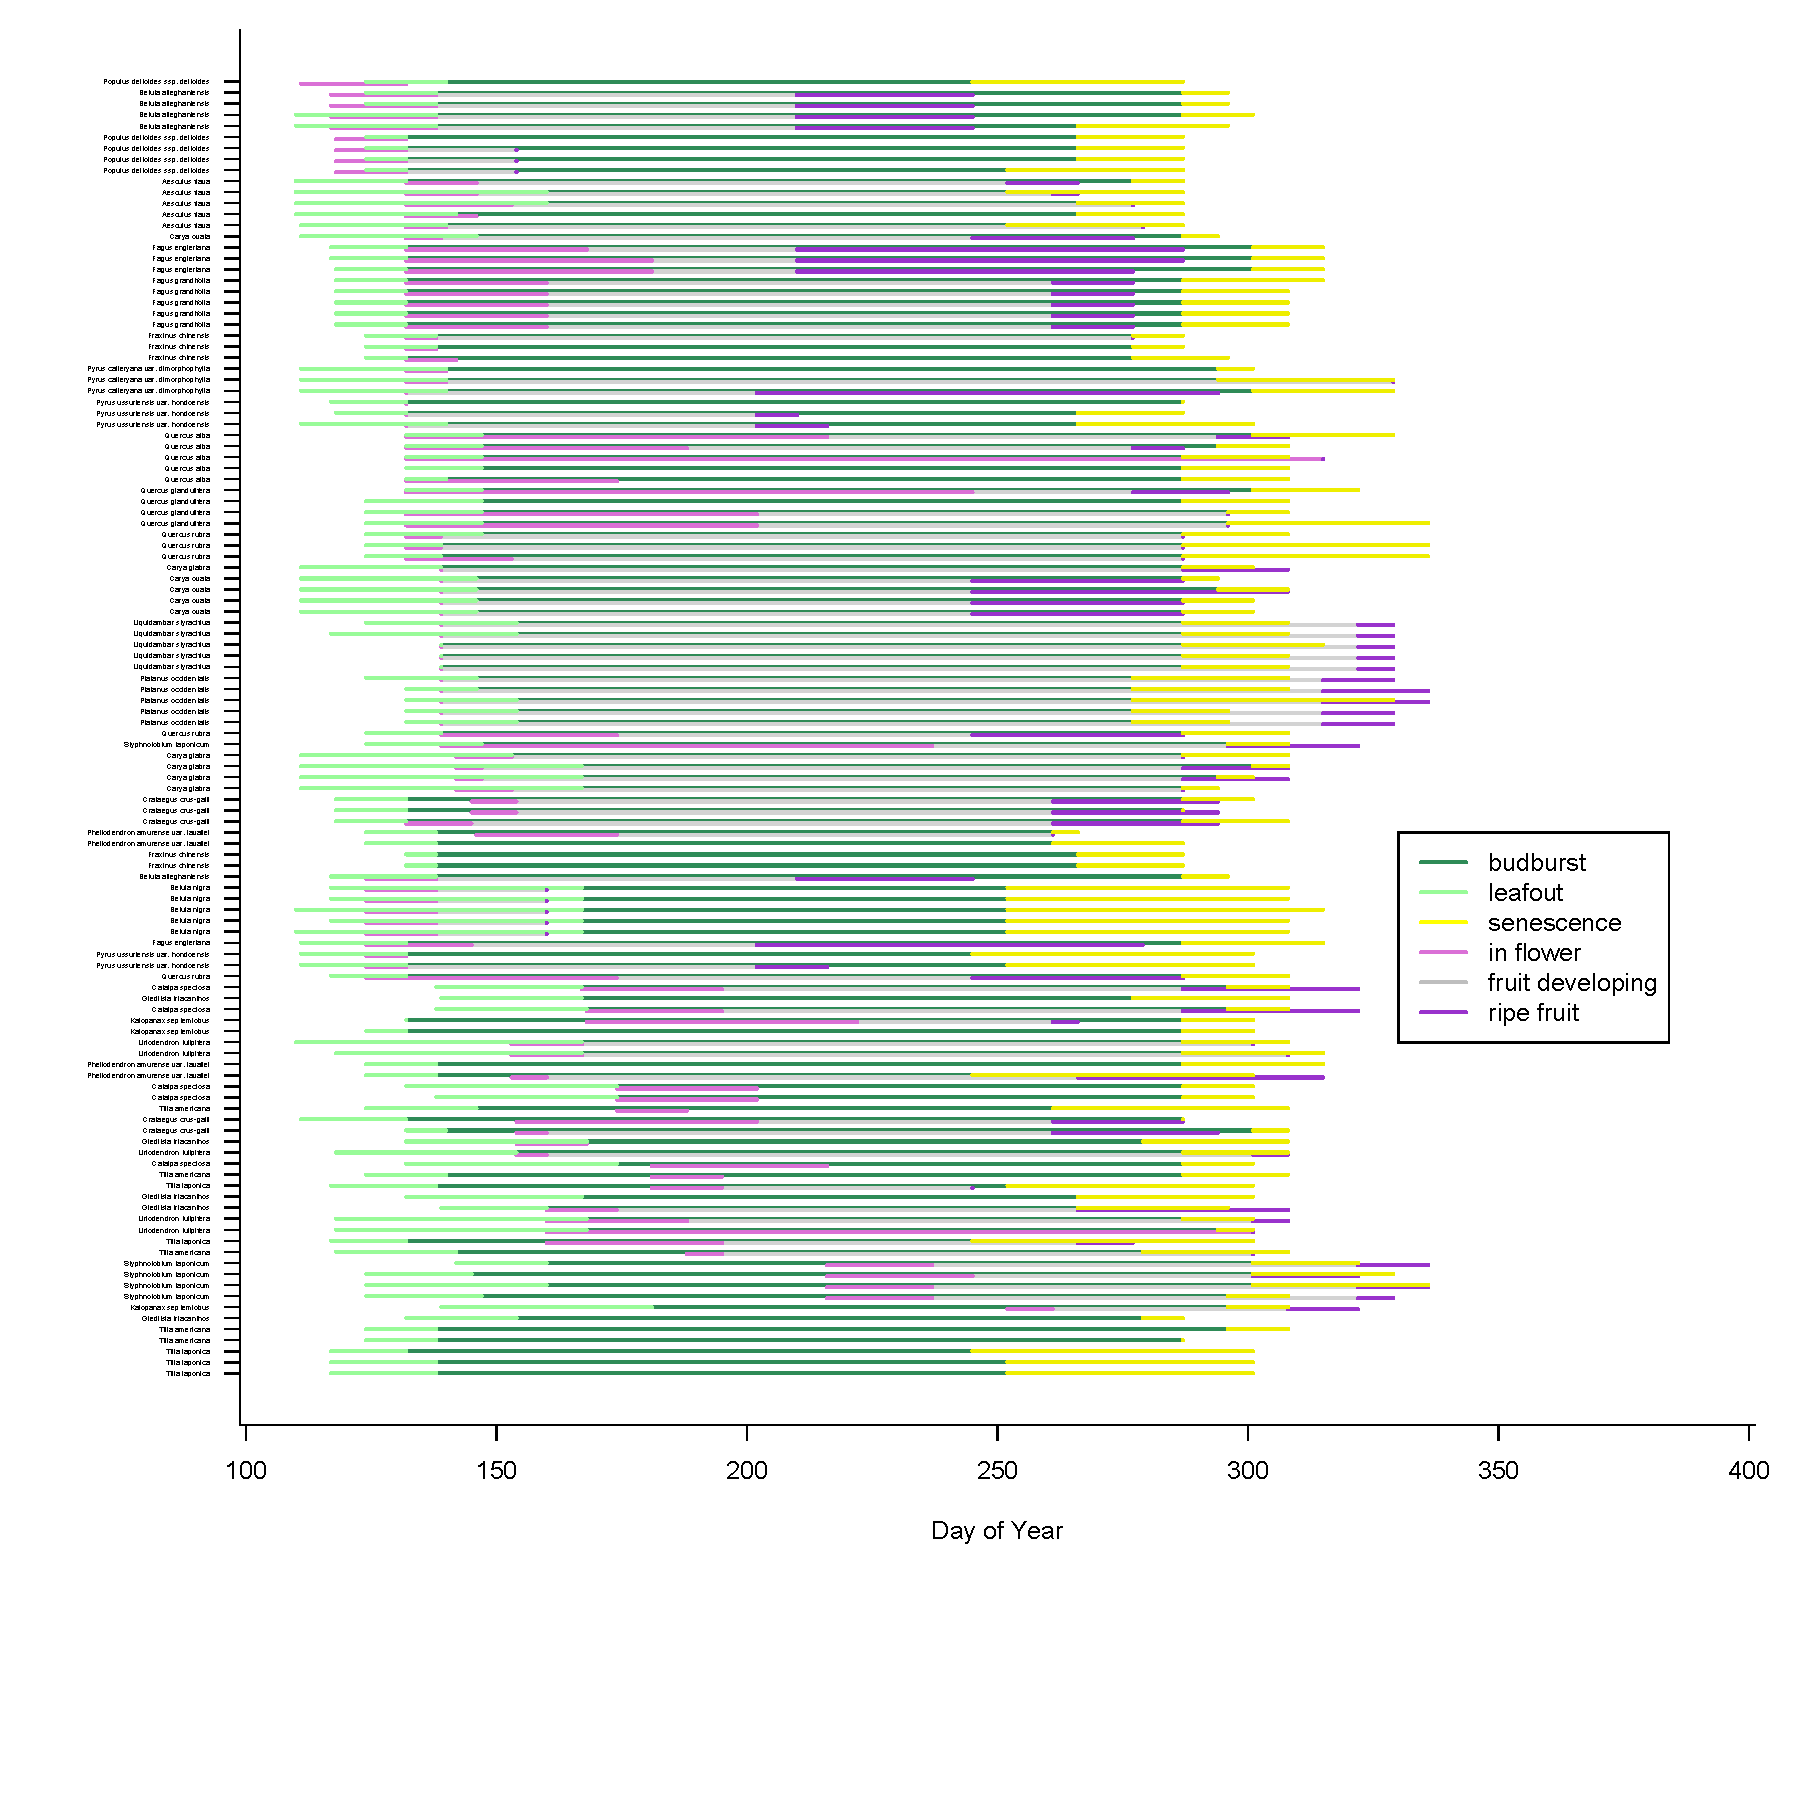
\includegraphics{../analyses/figures/grosea_repsort_ripefruit_ind_legend.pdf}
  \caption{\textbf{Individual tree phenology during the 2015 growing season, ordered by species-level mean first-flower dates.} Growth phenology is shown for budburst (from day-of-year it was first observed on the individual to the first day-of-year  leafoutwas observed), leafout (from the first day-of-year when fully-expanded leaves were observed through the first day senescence was observed), and senescence (from first day-of-year when leaves began changing color through the day-of-year when more than 95\% of leaves on the tree had changed color). Reproductive phenology is shown for flowering (from the first day-of-year when flowers appeared to the day-of-year when fruits first appeared, across all individuals within a species) and fruiting (from the first day-of-year when fruits appeared to the day-of-year when more than 95\% of fruits were first observed as ripe).}
 \label{fig:focind}
\end{figure}
\clearpage
 
%%%%%%%%%%%%%%%%%%%%%%%%%%%%%%%%%%%%%%%%
\end{document}
%%%%%%%%%%%%%%%%%%%%%%%%%%%%%%%%%%%%%%%%
